\section{Grundlagen}
\subsection{Allgemeine Grundlagen}
\subsubsection{Ganz schön clever}
Die folgende Abbildung zeigt das Spielbrett des Spiels "Ganz schön clever" zu dem im Rahmen dieser Arbeit eine KI implementiert werden soll:

\vspace{0.5cm}
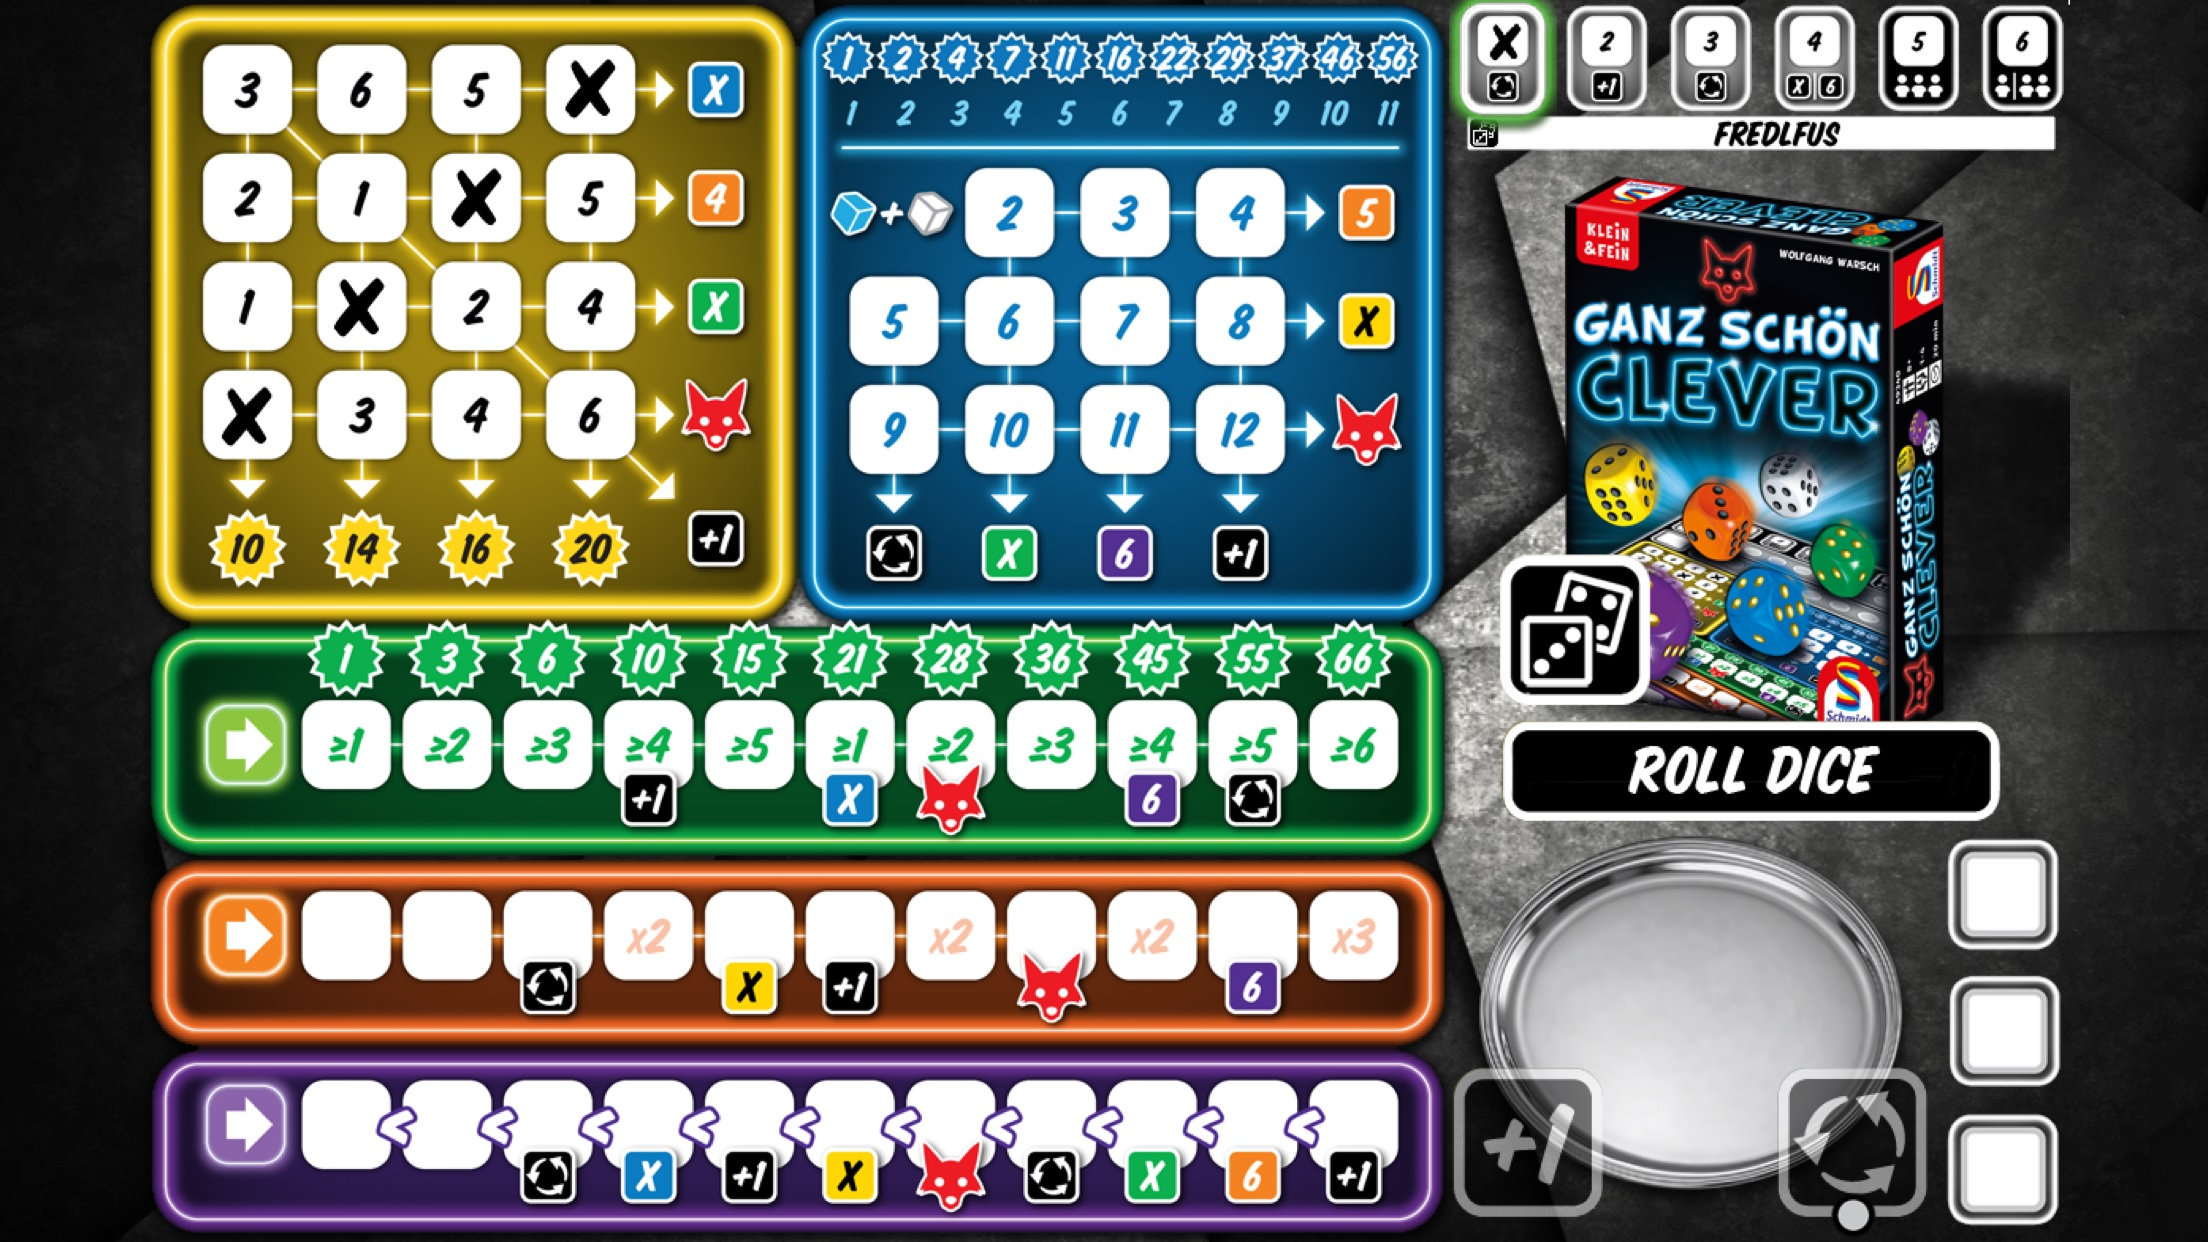
\includegraphics[width=1\textwidth]{Bilder/gsc} 

Abb. 1: Ganz schön clever 

Quelle: [Google Play Store, de.brettspielwelt.ganzschoenclever]\\


Im folgenden werden der Spielablauf und die wesentlichen Regeln des Spiels erklärt.

Es gibt sechs farbige Würfel, wobei jeder bis auf den weißen einem der 5 farbigen Spielfelder zuzuordnen ist. Der weiße Würfel ist ein Sonderwürfel und kann als einer anderen Würfel betrachtet werden. Wenn bestimmte Bedingungen erfüllt sind kann der Spieler einen Würfel wählen und das entsprechende Subfeld ausfüllen. Die Felder verfügen über Belohnungen, welche freigeschaltet werden, wenn eine bestimmte Kombination oder Anzahl an Feldern freigeschaltet worden ist. Beim orangenen und lila Feld kommt es bei der Belohnung zudem darauf an wie hoch das Würfelergebnis des gewählten Würfels ist, da die einzelnen Subfelder hier je nach Würfelergebnis zusätzlich belohnt werden.
\\
Das Spiel teilt sich in bis zu sechs Runden mit jeweils bis zu frei Würfen ein. Nach jeder Runde bekommt der Spieler zudem die Möglichkeit einen Würfel auf dem Tablett eines Mitspielers zu wählen. Diese Wahl verhält sich so wie bei der Wahl eines eigenen Würfels bei den Würfen des Spielers selbst. Die Anzahl der Runden werden von der Spielerzahl festgelegt. Bei ein bis zwei Spielern sind es sechs Runden. Bei drei Spielern sind es fünf Runden und bei vier Spielern sind es vier Runden. Die Anzahl der Würfe pro Runde ist immer drei, allerdings kann diese Anzahl reduziert werden, wenn kein Würfel mehr zum Würfeln zur Verfügung steht. Dann wird der Spielablauf fortgesetzt als hätte der Spieler seinen dritten Wurf in der Runde beendet und er kann einen Würfel vom Tablett des Mitspielers wählen bevor dann die neue Runde für ihn beginnt. Zu beginn der ersten, zweiten, dritten und vierten Runde bekommt jeder Spieler zudem eine Belohnung, welche oben rechts auf Abbildung 1 bei der jeweiligen Rundenzahl zu finden ist.
\\
Es gibt zwei Arten von Belohnungen im Spiel. Punktebelohnungen und Boni. Bei Punktebelohnungen handelt es sich um Punkte welche auf dem Score des Spielers addiert werden, welcher am Ende des Spiels entscheidet wer gewonnen hat. Der Spieler mit dem höchsten Score gewinnt das Spiel. Punktebelohnungen erhält man beim gelben Feld indem man eine Spalte vollständig ausfüllt. Die Anzahl der Punkte findet sich am Ende der Spalte. Im blauen Feld mit zunehmender Anzahl der ausgefüllten blauen Subfelder. Die Anzahl der Punkte findet sich oben im blauen Feld. Im grünen Feld ebenso mit zunehmender Anzahl der ausgefüllten grünen Subfelder. Die Anzahl der Punkte findet sich auch hier oben im grünen Feld. Im orangenen und lila Feld muss man dafür lediglich ein Subfeld ausfüllen. Die Punktebelohnung entspricht der Augenzahl des entsprechenden ausgefüllten Subfeldes. Beim orangenen Feld wird diese Augenzahl bei einigen Feldern zusätzlich mit zwei oder drei multipliziert. Außerdem gibt es eine Boni Belohnung, welche indirekt eine Punktebelohnung darstellt. Es handelt sich hierbei um den sogenannten Fuchs beziehungsweise die Füchse. Die Anzahl der freigeschalteten Füchse wird am Ende des Spiels mit der Anzahl der erzielten Punkte des Feldes mit den niedrigsten erreichten Punktewert multipliziert und zum Gesamtpunktestand addiert.

Bei Boni handelt es sich um Belohnungen, welche der Spieler nutzen kann oder muss um sich im Spiel einen Vorteil zu verschaffen. Die Boni sind bei den entsprechenden Subfeldern beziehungsweise am Rande von Spalten und Zeilen eingezeichnet und können freigeschaltet werden indem man diese ausfüllt. Eine Ausnahme bildet hier die Boni welche beim gelben Feld freigeschaltet wird indem alle diagonalen Felder von links oben nach rechts unten ausgefüllt werden. \\

Jede Boni hat ihr eigenes Symbol. Nun folgt eine Aufzählung und Erklärung der verschiedenen Boni mit Ausnahme der Füchse. Boni werden bei der Benutzung aufbraucht. Man kann mehr als eine dieser Boni auf einmal besitzen.

Extra Wahl: Bei der Extra Wahl wird es dem Spieler ermöglicht am Ende seiner Würfe beziehungsweise nachdem er einen Würfel vom Silbertablett des Gegners gewählt hat erneut Würfel zu wählen und die entsprechenden Felder dafür anzukreuzen. Würfel die so gewählt wurden können mithilfe der Extra Wahl Boni im selben Wurf nicht erneut gewählt werden. Es können alle Würfel gewählt werden, nicht nur die, welche unter normalen Umständen gültig zur Wahl stehen. Das Symbol ist die +1.

Neuer Wurf: Der Neue Wurf ermöglicht es dem Spieler einen seinen Würfe zu wiederholen ohne dabei einen der Würfel auszuwählen. Dies ermöglicht es ihm Würfe mit ungünstigen Ergebnissen neu auszurichten. Das Symbol sind die drei Pfeile die im Kreis angeordnet sind.

Gelbes Kreuz: Ermöglicht es dem Spieler direkt nach erhalten der Boni eines der gelben Subfelder nach eigener Wahl auszufüllen. Das Symbol ist ein Kreuz auf gelbem Hintergrund.

Blaues Kreuz: Ermöglicht es dem Spieler direkt nach erhalten der Boni eines der blauen Subfelder nach eigener Wahl auszufüllen. Das Symbol ist ein Kreuz auf blauem Hintergrund.

Grünes Kreuz: Ermöglicht es dem Spieler direkt nach erhalten der Boni das nächste freie Grüne Subfeld auszufüllen. Das Symbol ist ein Kreuz auf grünem Hintergrund.

Orangene Vier: Ermöglicht es dem Spieler direkt nach erhalten der Boni das nächste freie orangene Subfeld mit einer vier auszufüllen. Das Symbol ist eine vier auf orangenem Hintergrund.

Orangene Fünf: Ermöglicht es dem Spieler direkt nach erhalten der Boni das nächste freie orangene Subfeld mit einer fünf auszufüllen. Das Symbol ist eine fünf auf orangenem Hintergrund.

Orangene Sechs: Ermöglicht es dem Spieler direkt nach erhalten der Boni das nächste freie orangene Subfeld mit einer sechs auszufüllen. Das Symbol ist eine sechs auf orangenem Hintergrund.

Lila Sechs: Ermöglicht es dem Spieler direkt nach erhalten der Boni das nächste freie lila Subfeld mit einer sechs auszufüllen. Das Symbol ist eine sechs auf lila Hintergrund. \\

Nun folgen die Regeln nach denen bestimmt wird ob ein Würfel gewählt werden kann um ein Subfeld auszufüllen und ob er ein gültiger Würfel ist:

Ist ein Würfel ungültig kann dieser auch nicht gewählt werden. Würfel werden ungültig indem sie in dieser Runde bereits gewählt worden sind. Außerdem werden Würfel, welche eine geringere Augenzahl aufweisen als der aktuell gewählte Würfel auch automatisch ungültig. Eine Ausnahme ist hierbei die Wahl eines Würfels vom Silbertablett des Gegenspieler oder Wahlen von Würfeln durch die Extra Wahl Boni. Würfel werden wieder gültig am Anfang der Runde, nach Abschluss des dritten Wurfes (beinhaltet Wahl des Würfels), sowie nachdem Wahlen mit dem Extra Wahl Boni erfolgt sind.

Jedes Feld hat seine eigenen Regeln, die bestimmen, wann ein Subfeld ausgefüllt werden darf. Beim gelben Feld muss die Augenzahl des Würfel mit der Zahl des Subfeldes übereinstimmen. Beim Blauen Feld muss die Summe der Augenzahlen des blauen und des weißen Würfels mit der Zahl des Subfeldes übereinstimmen. Beim grünen Feld muss die Augenzahl des Würfels größer oder gleich der Zahl im Subfeld sein. Zudem kann immer nur das nächste freie Feld ausgefüllt werden, beginnend von links. Im orangenen Feld kann immer das nächste Subfeld eingetragen werden. Auch hier beginnend von links. Beim lila Feld muss die Augenzahl des Würfels größer sein als die Zahl im zuletzt ausgefüllten Subfeld. Eine Ausnahme bildet hier der Fall in dem eine sechs im zuletzt ausgefüllten Subfeld steht. Dann kann das nächste Feld mit jeder beliebigen Augenzahl gewählt werden. Die sechs setzt die Voraussetzung für das lila Feld bis zum nächsten ausfüllen sozusagen aus. Auch hier gilt die Reihenfolge von links nach rechts.
\subsubsection{Machine Learning}
"Maschinelles Lernen heißt, Computer so zu programmieren, dass ein bestimmtes Leistungsmerkmal anhand von Beispieldaten oder Erfahrungswerten optimiert wird" [Maschinelles Lernen, Seite 3].

Es gibt bis heute nach wie vor viele Problemstellungen, die von Menschen auf einfache Art und weise lösbar sind, für die es aber keine Algorithmische Lösung zu geben scheint. Hier kommt das maschinelle Lernen zum Einsatz. Durch die Mustererkennung aus Trainingsdaten können Programme lernen solche Problemstellungen zu lösen indem sie präzise Vorhersagen über bestehende Sachverhalte aus beliebigen Daten des selben oder eines ähnlichen Sachverhaltes, der beim Training vorhanden war, zu treffen. Ein besonders weit verbreiteter Anwendungsfall ist die Herleitung von Kundenverhalten und möglicher Optimierungsmöglichkeiten für den Verkauf. Wenn man ein Programm mithilfe von maschinellem Lernen trainiert hat, nennt man dieses dann Modell. Ein solches Modell wird häufig erst auf allgemeinen Datensätzen und später auf immer spezifischeren trainiert, sodass es schließlich auf eine konkrete Aufgabe zugeschnitten werden kann [Maschinelles Lernen, Seite 1f].

Maschinelles Lernen ermöglicht es zwar nicht einen gesamten Prozess mit all seinen Einzelheiten zu verstehen, aber es ermöglicht relevante Merkmale zu erkennen und Schlüsse über den gesamten Sachverhalt zu schließen und auf Grund dessen zu agieren zu können oder zumindest Vorhersagen über diesen zu treffen [ML, Seite 2].

Die Anwendungsgebiete von maschinellem Lernen sind zahlreich. Unter anderem ist es relevant für den Einzelhandel und Finanzdienstleister, um Kreditgeschäfte abzuwickeln, Betrugsversuche zu erkennen, oder den Aktienmark einzuschätzen. Aber auch Fertigung wird es zur Optimierung, Steuerung und Fehlerbehebung eingesetzt. Auch in der Medizin erweisen sich medizinische Diagnoseprogramme mithilfe von Modellen, die mit maschinellem Lernen trainiert wurden als nützlich [ML, Seite 3].

 Und das sind nur einige wenige der möglichen Bereiche in denen maschinelles Lernen bereits Anwendung findet. 
 
 Die Datenbestände und das World Wide Web werden immer größer und die Suche nach relevanten Daten kann nicht mehr manuell vorgenommen werden [ML, Seite 3].
 
 "Das maschinelle Lernen ist aber nicht nur für Datenbanken relevant, sondern auch für das Gebiet der künstlichen Intelligenz" [ML, Seite 3].
 
 Von Intelligenz spricht man dann, wenn das System selbstständig in einer sich verändernden Umgebung lernen und sich anpassen kann. Dadurch muss der Systementwickler nicht jede erdenkliche Situation vorhersehen und passende Lösungen dafür entwickeln [ML, Seite 3].
 
 Maschinelles Lernen findet seine Anwendung in dieser Arbeit in Form von Deep Reinforcement Learning. Was Reinforcement Learning ist und wie es sich von Deep Reinforcement Learning unterscheidet wird im Folgenden beschrieben.
\subsubsection{Reinforcement Learning}
Reinforcement Learning (im deutschen Bestärkendes Lernen) heißt so, weil es die Aktionen des Agenten (beziehungsweise des Modells) bestärkt. Man kann sich das in etwa so vorstellen, wie das Training eines Hundes im Park. Dieser wird jedes mal wenn er einen Trick richtig ausführt mit einem Leckerli belohnt. Diese Belohnung bestärkt das Verhalten des Hundes und das Tier lernt dieses in Zukunft zu wiederholen. Eine negative Aktion kann hingegen bestraft werden, damit sie in Zukunft nicht wiederholt wird [RL, Seite 11].

Im Reinforcement Learning sind vor allem Folgende Begriffe wichtig:

Agent (oder Modell): Dabei handelt es sich um die Entität, welche mit der Umgebung interagiert und die Entscheidungen trifft. Dabei kann es sich zum Beispiel um einen Roboter oder autonomes Fahrzeug handeln [RL, Seite 11]. In dieser Arbeit ist diese Entität ein Modell, welches mithilfe der Bibliothek Stable-Baselines3 erstellt wird.

Umgebung: Dabei handelt es sich um die Außenwelt des Agenten [RL, Seite 11]. der Agent interagiert mit dieser und erhält je nach Zustand der Umgebung und seiner gewählten Aktion ein entsprechendes Feedback.

Aktion: Eine Aktion beschreibt das Verhalten des Agenten [RL, Seite 11]. In dieser Arbeit wählt der Agent Felder des Spielbrettes zum ausfüllen als Aktionen aus. Außerdem entscheidet er ob er bestimmte Boni nutzen möchte oder nicht.

Zustand: Der Zustand beschreibt den Zusammenhang zwischen Umgebung und Agent [RL, Seite 11]. In dieser Arbeit ist der Zustand von den Eigenschaften des Spielbrettes, der Würfel, der Rundenanzahl und der erspielten Boni abhängig.

Belohnung: Positive oder negative Vergeltung je nachdem wie gut der Zustandswechsel von Zustand x nach Zustand y gewesen ist [RL, Seite 11]. In dieser Arbeit wird dies durch die jeweiligen Punktebelohnungen im Spiel verkörpert. Eine Ausnahme bildet hier eine negative Belohnung, wenn der Agent in einen Zustand gerät in dem er keine gültige Aktion tätigen kann.

Policy: Die Policy ist die Strategie des Agenten, nach welcher er seine nächsten Aktionen wählt [RL, Seite 11]. In dieser Arbeit wird die Policy durch ein Multilayer Perceptron (siehe Deep Learning) abgebildet.

Episode: Eine Menge an Zusammenhängenden Aktionen, welche endet, wenn das Ziel erreicht worden ist [RL, Seite 11]. In dieser Arbeit ist eine Episode ein kompletter Spieldurchlauf von Ganz schön clever.


Die folgende Abbildung beschreibt einen Lernzyklus im Reinforcement Learning:

\vspace{0.5cm}
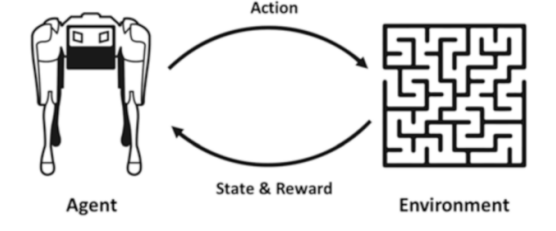
\includegraphics[width=0.8\textwidth]{Bilder/rl}

Abb. 2: Reinforcement Learning

Quelle: [RL, Seite 12]\\


Der Agent führt eine Aktion in der Umgebung aus und erhält daraufhin eine Belohnung und den neuen Zustand der Umgebung als Feedback. Daraufhin aktualisiert er seine Policy, um in Zukunft bessere Aktionen tätigen zu können.

Hierbei ist das Ziel des Agenten die gesamte erreichte Belohnung zu maximieren. Demnach wird die Policy dementsprechend angepasst, dass dies begünstigt wird [RL, Seite 12f].

Doch dabei gibt es einiges Schwierigkeiten, die es zu beachten gilt. Belohnungen die in kurzer Zeit erreicht werden können, könnten wichtiger oder weniger wichtig sein als Belohnungen, die erst innerhalb vieler Schritte erreicht werden können. Ein gutes Beispiel hierfür wäre ein Balanceakt, bei dem es besonders wichtig ist kurzzeitige Belohnungen zu bevorzugen, da die Episode endet, wenn das Balancieren fehlschlägt, was eine starke negative Belohnung zur Folge haben kann.

Ein weiterer Faktor ist die Balance zwischen Erkundung und Ausbeutung. Diese zwei Prinzipien sind wesentlich für das Reinforcement Learning. Dabei geht es darum, wie stark die Policy es vorzieht neue oder selten gesehene Zustände und Aktionen auszuprobieren oder bereits bekannte, welche eine gute Belohnung zu bringen scheinen auszunutzen beziehungsweise auszubeuten [RL, Seite 13].
\subsubsection{Deep Learning}
Was unterscheidet Reinforcement Learning von Deep Reinforcement Learning? Im wesentlichen handelt es sich um das selbe Konzept, allerdings ist das eine Deep Learning und das andere nicht. Was ist also Deep Learning?

Von Deep Learning spricht man sobald ein Neuronales Netz mehrere versteckten Schichten hat. 

Ein solches Netz besteht aus einer Vielzahl von Neuronen. [DRL, Seite 75] Ein solches Neuron setzt sich zusammen aus Inputs, Outputs, Gewichtungen dieser In- und Outputs, sowie einer Aktivierungsfunktion, welche auch gewichtet sein kann. Ein Spezialfall eines solchen Neuronalen Netzes ist ein sogenanntes Multilayer Perceptron. Bei diesem sind alle Neuronen in einer Schicht mit allen Neuronen der folgenden Schicht verbunden. Häufig haben auch alle Neuronen der versteckten Schichten die selbe Aktivierungsfunktion. Was den Beitrag der einzelnen Neuronen zum Gesamtergebnis des Netzes steuert sind im wesentlichen die unterschiedlichen Gewichtungen der Neuronen und ihre Position im Netz.

\begin{minipage}{\linewidth}
	Die folgende Abbildung zeigt ein solches Multilayer Perceptron:
	
	\vspace{0.5cm}
	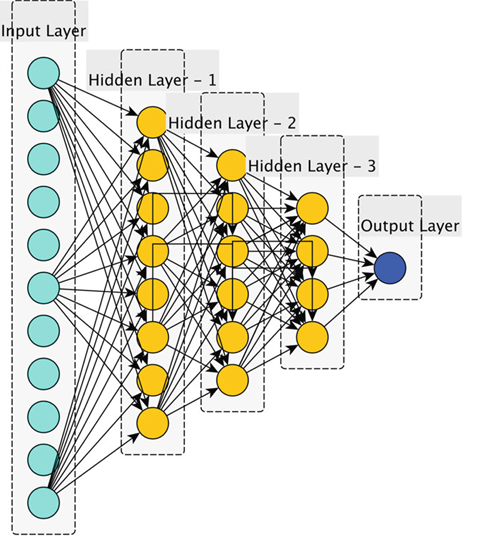
\includegraphics[width=0.8\textwidth]{Bilder/mlp} 
	
	Abb. 3: Multilayer Perceptron
	
	Quelle: [DRL, Seite 78]\\
\end{minipage}


Die Inputs des Netzes sind die Werte von Variablen der zur Verfügung stehenden Beobachtungen der Umgebung. Die versteckten Schichten verarbeiten diese Inputs dann mit ihren Funktionen und Gewichtungen. Das Output des Netzes ist hingehen eine Gewünschte Vorhersage, die mit ihrer eigenen Aktivierungsfunktion hergeleitet wird.
\subsubsection{Proximal Policy Optimization}
Proximal Policy Optimization oder kurz PPO ist eine neue Policy Gradient Methode für Reinforcement Learning. Im Gegensatz zu standardmäßigen Policy Gradient Methoden ist es mit dieser Methode möglich mehrere Policy Updates pro Datenpaket durchzuführen. PPO hat einige der Vorteile der Trusted Region Policy Optimization (kurz TRPO), ist aber simpler zu implementieren und hat auch andere Vorteile, wie bessere Generalisierbarkeit und niedrigere Stichproben Komplexität. PPO zeigt eine gute Balance zwischen Stichproben Komplexität, Einfachheit und Trainingsgeschwindigkeit [PPO, Seite 1].

Die Stichprobenkomplexität beschreibt wie groß ein Datenpaket sein muss, um dem Algorithmus ein gewisses Level an Performance zu ermöglichen. Dies ermöglicht es mehr Updates mit weniger Gesamtdaten durchzuführen, was vor allem hilfreich ist, wenn nicht genügend Daten zur Verfügung stehen.

Policy Gradient Methoden berechnen einen Gradienten und passen die Policy in Richtung der negativen Steigung an. Das kann man sich ähnlich wie einen Punkt auf einer Parabel vorstellen, die Policy entspricht dem Punkt und wird so lange angepasst beziehungsweise verschoben, bis sie möglichst das Minimum der Parabel erreicht.

Bei der Trusted Region Policy Optimization gibt es eine vertrauenswürdige Region innerhalb die Policy abgeändert werden darf. Das soll sicherstellen, dass die Policy nicht zu stark abgeändert wird, um ein stabileres Training zu gewährleisten. Im Gegensatz zur PPO werden Änderungen, die zu stark abweichen verworfen.

Bei der PPO kommt es zum sogenannten Clipping. Hierbei werden zu starke Änderungen abgeschnitten im übertragenen Sinne und es kommt zu einer abgeschwächten Änderung der Policy.

PPO ist ein verhältnismäßig simpler, einfach verstehender und dennoch effizienter Algorithmus. Er hat eine gute Balance zwischen Stabilität und Effizienz. Außerdem erzielt er gute Ergebnisse bei einer großen Bandbreite an Aufgaben. Daher eignet sich PPO besonders gut für Einsteiger, die bisher nicht viel mit Deep Reinforcement Learning gearbeitet haben.
\subsection{Verwendete Technologien}
\subsubsection{Gymnasium}
\subsubsection{Stable Baselines 3}
\subsubsection{Matplotlib}
\subsubsection{ChatGPT 4}